\documentclass[12pt, letterpaper]{article}
\usepackage[english]{babel}
\usepackage{adjustbox}
\usepackage[utf8]{inputenc}  
\usepackage{csquotes}
\usepackage[authordate,backend=biber]{biblatex-chicago}
\usepackage[margin=1in]{geometry}
\usepackage{abstract, multirow, pdflscape, floatrow, parskip, fancyhdr, amsmath, tabularx, tabu, titlesec}
\usepackage{float, array, indentfirst, amssymb, titlesec, hyperref, longtable, listings, makecell}
\usepackage[format=plain,up,textfont=normal,up,justification=justified,singlelinecheck=false]{caption} 
\usepackage[bottom,flushmargin,hang]{footmisc}
\usepackage{amsmath}
\usepackage{pgfplots}
\pgfplotsset{compat = newest}
\usepackage{abstract, amsmath, amssymb, array, indentfirst, fancyhdr, floatrow, listings, longtable, multirow, biblatex, pdflscape, setspace, tabu, tabularx, titlesec, url}
\usepackage{booktabs,wrapfig}
\usepackage{siunitx}
\newcolumntype{d}{S[
	input-open-uncertainty=,
	input-close-uncertainty=,
	parse-numbers = false,
	table-align-text-pre=false,
	table-align-text-post=false
	]}
\usepackage{tikz}
\newcommand*\circled[1]{\tikz[baseline=(char.base)]{
		\node[shape=circle,draw,inner sep=2pt] (char) {#1};}}
\usepackage{fancyhdr} 
%\usepackage[justification=centering]{caption}
\usepackage[final]{pdfpages}
\usepackage{floatrow}
\captionsetup[table]{singlelinecheck=false,justification=centering,position=bottom}
\captionsetup[figure]{singlelinecheck=false,justification=centering,position=bottom}
\hypersetup{colorlinks=false,
	pdfborder={0 0 0},}
\setlength{\parindent}{24pt}
\newcommand{\forceindent}{\leavevmode{\parindent=2em\indent}}
\lstset{basicstyle=\ttfamily, columns=flexible, breaklines=true}
\fancyhf{}

\renewcommand{\arraystretch}{1.2}

\fancyfoot[C]{\footnotesize\thepage}
\newcolumntype{R}{>{\raggedright\arraybackslash}X}
\titleformat{\title}{\section}{\large\bfseries}{\thesection}{1em}{}
\setlength{\parskip}{0pt}
\doublespacing

%\addbibresource{rn.bib}

%%%%%%%%%%%%%%%%%%%%%%%%%%%%%%%%

\titleformat*{\section}{\large\bfseries}
%\usepackage{fancyhdr}
%\pagestyle{fancy}
%\fancyhead{}
%\fancyhead[CO]{\textbf{\small Page UNO}}
%\fancyhead[CE]{\textbf{\small Page DOS }}
%\fancyfoot[CO]{Compiled: \textit{\today}}
%\fancyfoot[CE]{Compiled: \textit{\today}}
%\fancyhead[RO, LE]{\textbf{\small\thepage}}
%\renewcommand{\headrulewidth}{0pt} \renewcommand{\footrulewidth}{0pt}
\setlength{\parindent}{3em}

\title{\large \textbf{XXX}}

% Authors listed in order of contribution
\author{XXX}

\date{\today}

\begin{document}
	%\setcounter{secnumdepth}{0}
	
	% Render title
	\maketitle
	\thispagestyle{empty}
	\vspace{4cm}
	
	% Abstract
	\begin{abstract}
		\vspace{0.25cm}\noindent XXX
	\end{abstract}
	
	\pagebreak
	
\setlength{\parindent}{1cm}
\parskip=0pt
\setcounter{page}{1}

\subsection*{Data and Variables}

\begin{table}[htbp] \centering 
	\caption{Summary statistics for the main variables} 
	\label{t1} 
	\begin{tabular}{@{\extracolsep{5pt}}lccccc} 
		\\[-1.8ex]\hline 
		\hline \\[-1.8ex] 
		Variable & \multicolumn{1}{c}{N} & \multicolumn{1}{c}{Mean} & \multicolumn{1}{c}{SD} & \multicolumn{1}{c}{Min.} & \multicolumn{1}{c}{Max.} \\ 
		\hline \\[-1.8ex] 
		Civilian targeting & 170 & 0.365 & 0.483 & 0 & 1 \\ 
		Inclusive service provision & 132 & 0.182 & 0.387 & 0 & 1 \\ 
		Secessionist aim & 169 & 0.272 & 0.446 & 0 & 1 \\ 
		Territorial control & 168 & 0.357 & 0.481 & 0 & 1 \\ 
		Communist ideology & 170 & 0.176 & 0.382 & 0 & 1 \\ 
		Foreign support & 159 & 0.566 & 0.497 & 0 & 1 \\ 
		\hline \\[-1.8ex] 
	\end{tabular} 
\end{table} 

\subsection*{Results}

\begin{figure}[htbp]
	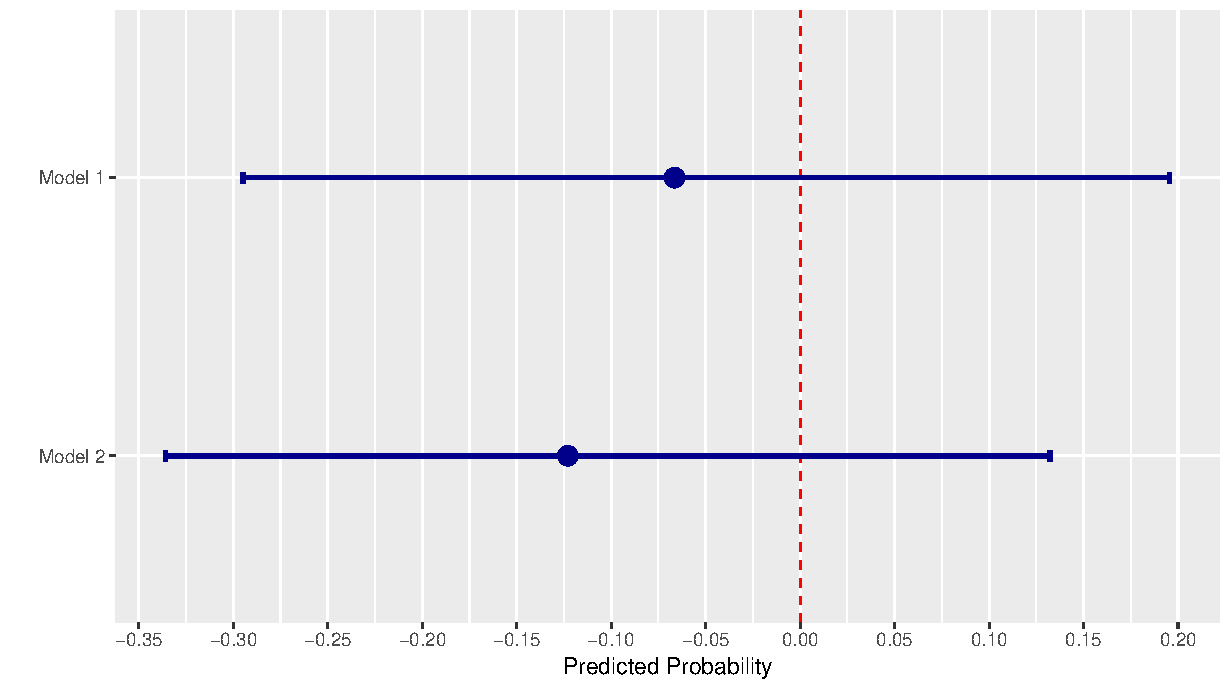
\includegraphics[scale=.7]{predplot.pdf}
	\caption{Mean simulated predicted probabilities and 95\% CIs}\label{f1}
\end{figure}

%\clearpage

%\pagebreak
%\begingroup
%\titleformat*{\section}{\fontsize{14pt}{18pt}\bfseries\selectfont}
%\printbibliography
%\endgroup

\end{document}